%%%%%%%%%%%%%%%%%%%%%%%%%%%%%%%%%%%%%%%%%
% Beamer Presentation
% LaTeX Template
% Version 1.0 (10/11/12)
%
% This template has been downloaded from:
% http://www.LaTeXTemplates.com
%
% License:
% CC BY-NC-SA 3.0 (http://creativecommons.org/licenses/by-nc-sa/3.0/)
%
%%%%%%%%%%%%%%%%%%%%%%%%%%%%%%%%%%%%%%%%%

%----------------------------------------------------------------------------------------
%	PACKAGES AND THEMES
%----------------------------------------------------------------------------------------

\documentclass{beamer}

\mode<presentation> {

% The Beamer class comes with a number of default slide themes
% which change the colors and layouts of slides. Below this is a list
% of all the themes, uncomment each in turn to see what they look like.

%\usetheme{default}
%\usetheme{AnnArbor}
%\usetheme{Antibes}
%\usetheme{Bergen}
%\usetheme{Berkeley}
%\usetheme{Berlin}
%\usetheme{Boadilla}
\usetheme{CambridgeUS}
%\usetheme{Copenhagen}
%\usetheme{Darmstadt}
%\usetheme{Dresden}
%\usetheme{Frankfurt}
%\usetheme{Goettingen}
%\usetheme{Hannover}
%\usetheme{Ilmenau}
%\usetheme{JuanLesPins}
%\usetheme{Luebeck}
%usetheme{Madrid}
%\usetheme{Malmoe}
%\usetheme{Marburg}
%\usetheme{Montpellier}
%\usetheme{PaloAlto}
%\usetheme{Pittsburgh}
%\usetheme{Rochester}
%\usetheme{Singapore}
%\usetheme{Szeged}
%\usetheme{Warsaw}

% As well as themes, the Beamer class has a number of color themes
% for any slide theme. Uncomment each of these in turn to see how it
% changes the colors of your current slide theme.

%\usecolortheme{albatross}
%usecolortheme{beaver}
%\usecolortheme{beetle}
%\usecolortheme{crane}
%\usecolortheme{dolphin}
%\usecolortheme{dove}
%\usecolortheme{fly}
%\usecolortheme{lily}
%usecolortheme{orchid}
%\usecolortheme{rose}
%\usecolortheme{seagull}
\usecolortheme{seahorse}
%\usecolortheme{whale}
%\usecolortheme{wolverine}

%\setbeamertemplate{footline} % To remove the footer line in all slides uncomment this line
%\setbeamertemplate{footline}[page number] % To replace the footer line in all slides with a simple slide count uncomment this line

\setbeamertemplate{navigation symbols}{} % To remove the navigation symbols from the bottom of all slides uncomment this line
}
%\usepackage[brazilian]{babel}
\usepackage[utf8]{inputenc}
\usepackage{pgfplots}
\usepackage{graphicx} % Allows including images
\usepackage{booktabs} % Allows the use of \toprule, \midrule and \bottomrule in tables
\usepackage{courier}

%----------------------------------------------------------------------------------------
%	TITLE PAGE
%----------------------------------------------------------------------------------------

\title[EP3]{EP3 de MAC0422} % The short title appears at the bottom of every slide, the full title is only on the title page

\author{Gabriel Capella (8962078) e Luís Felipe de Melo Costa Silva (9297961)} % Your name
\institute[USP] % Your institution as it will appear on the bottom of every slide, may be shorthand to save space
{
IME-USP\\ % Your institution for the title page
\medskip
}

\begin{document}

\begin{frame}
\titlepage % Print the title page as the first slide
\end{frame}

%----------------------------------------------------------------------------------------
%	PRESENTATION SLIDES
%----------------------------------------------------------------------------------------

%------------------------------------------------
%\section{Problema} % Sections can be created in order to organize your presentation into discrete blocks, all sections and subsections are automatically printed in the table of contents as an overview of the talk
%------------------------------------------------

%\subsection{Subsection Example} % A subsection can be created just before a set of slides with a common theme to further break down your presentation into chunks

\begin{frame}
	\frametitle{Problema}
	\begin{itemize}
		\item Implementar um simulador de gerência de memória com diversos algoritmos para gerência do espaço livre e para substituição de páginas.
		\item Os algoritmos de gerência de espaço livre são:
		\begin{enumerate}
			\item First Fit
			\item Next Fit
			\item Best Fit
			\item Worst Fit
		\end{enumerate}
		\item Os algoritmos de substituição de página são:
		\begin{enumerate}
			\item Optimal
			\item Second-Chance
			\item Clock
			\item LRU (Quarta Versão)
		\end{enumerate}
	\end{itemize}
\end{frame}

\begin{frame}
	\frametitle{Implementação}
	\begin{itemize}
		\item A linguagem escolhida foi Python (versão 3.5.2 - \texttt{python3}), que é orientada a objetos e é uma linguagem de script ao mesmo tempo.
		\item Isso facilitou bastante a leitura do arquivo de trace, no armazenamento das informações, na alocação e desalocação da memória utilizada na execução do programa e no tratamento dos objetos durante os trabalhos.
	\end{itemize}
\end{frame}

%------------------------------------------------
\begin{frame}
	\frametitle{Módulos}
	\framesubtitle{ep3.py}
	\begin{itemize}
		\item Implementa o console no terminal, a interação com o usuário.
		\item É um envelope. Apenas lê as informações e então chama as funções responsáveis pelo comando lido.
		\item Os comandos são os que foram definidos pelo enunciado (\texttt{carrega}, \texttt{espaco}, \texttt{substitui}, \texttt{executa} e \texttt{sai}), com os respectivos argumentos.
		\item Utiliza a biblioteca \texttt{cmd} do Python.
		\item Depende do arquivo gerenciador.py
	\end{itemize}
\end{frame}

\begin{frame}
	\frametitle{Módulos}
	\framesubtitle{gerenciador.py}
	\begin{itemize}
		\item Faz o trabalho pesado pedido pelo módulo anterior (possui as funções que ele chama).
		\item Possui as seguintes funções:
		\begin{itemize}
			\item Leitura do arquivo de trace.
			\item Escolha do algoritmo de gerência de espaço livre e do algoritmo de substituição de página.
			\item Execução do simulador com as informações recebidas.
		\end{itemize}
		\item Depende dos módulos proccess.py e substitui.py
	\end{itemize}
\end{frame}

\begin{frame}
	\frametitle{Módulos}
	\framesubtitle{substitui.py}
	\begin{itemize}
		\item Possui duas classes: \texttt{Pagina} e \texttt{Substitui}.
		\item A classe \texttt{Pagina} inicializa o objeto \texttt{Pagina} com as seguintes informações: qual memória ela está, o número do processo, o número que o processo enxerga, o bit R, a próxima referência (para o Optimal), onde ele está na memória e quando ela foi chamada pela última vez.
		\item A classe \texttt{Substitui} possui as seguintes funções:
		\begin{itemize}
			\item Impressão de informações no console.
			\item Atribuição das informações lidas no console.
			\item Função que tira um processo pronto da fila.
			\item Configuração do bit R.
			\item Page fault (tem os algoritmos de substituição).
			\item Acesso à "memória."
		\end{itemize}
		\item Depende dos arquivos espaco.py, process.py e gerenciador\textunderscore arquivo.py
	\end{itemize}
\end{frame}

\begin{frame}
	\frametitle{Módulos}
	\framesubtitle{substitui.py}
	\begin{itemize}
		\item Nesse módulo temos uma lista de unidades de alocação.
		\item Quando um processo solicita acesso a alguma posição da memória $x$, calculamos $\left \lceil{\frac{x}{s}}\right \rceil$ para descobrir a página que o processo quer acessar.
		\item Exemplo: Seja $x = 82$ e $s = 4$, $\left \lceil{\frac{x}{s}}\right \rceil = 20$. 
		\item Usando o exemplo, procuramos se alguma unidade de alocação já apresenta a página 20 e seja desse processo.
		\item Se existir uma unidade que satisfaça o requisito, tentamos passá-la para a memória física.
		\item Se não existir, a criamos na memória virtual e então tentamos passá-la para a memória física.
	\end{itemize}
\end{frame}

\begin{frame}
	\frametitle{Módulos}
	\framesubtitle{process.py}
	\begin{itemize}
		\item Possui a definição do objeto \texttt{process}, que armazena as seguintes informações:
		\begin{itemize}
			\item PID
			\item Nome do processo
			\item Início e fim
			\item Páginas que ele acessa
			\item Quando acessa cada página.
		\end{itemize}
	\end{itemize}
\end{frame}

\begin{frame}
	\frametitle{Módulos}
	\framesubtitle{gerenciador\textunderscore arquivo.py}
	\begin{itemize}
		\item Esse arquivo cuida de escrever nos arquivos \texttt{/tmp/ep3.men} e \texttt{/tmp/ep3.vir}. Caso não existam, são criados.
		\item Possui as funções:
		\begin{itemize}
			\item Cria os arquivos e os enche com $-1$.
			\item Escreve em \texttt{/tmp/ep3.men}.
			\item Escreve em \texttt{/tmp/ep3.vir}
		\end{itemize}
		\item \textbf{Debug}: Para ver o que os arquivos representam, basta executar o comando \texttt{od -i -v tmp/ep3.men} ou \texttt{od -i -v tmp/ep3.vir} 
	\end{itemize}
\end{frame}

\begin{frame}
	\frametitle{Módulos}
	\framesubtitle{espaco.py}
	\begin{itemize}
		\item Esse módulo tem os algoritmos de gerência de memória implementados.
		\item Basicamente, possui duas funções:
		\begin{itemize}
			\item Devolver um endereço de espaço (usando o algoritmo escolhido).
			\item Liberar um espaço de memória que não será mais usado.
		\end{itemize}
		\item Tanto a memória física quanto a virtual implementadas utilizam esse módulo.
	\end{itemize}
\end{frame}

\begin{frame}
	\frametitle{Entrada}
	\begin{itemize}
		\item O módulo do console trabalha com essa parte.
		\item Um exemplo está abaixo:
		\begin{figure}[!h]
			\centering
			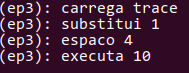
\includegraphics[scale=0.75]{a.png}
		\end{figure}
		\item Como podemos ver, o arquivo trace será lido, o algoritmo de substituição de página utilizado será o Optimal, o de gerenciamento de espaço livre será o Worst Fit e a impressão da execução será de 10 em 10 "segundos".
	\end{itemize}
\end{frame}

\begin{frame}
	\frametitle{Saída}
	\begin{itemize}
		\item A imagem abaixo é um exemplo de saída:
		\begin{figure}[!h]
			\centering
			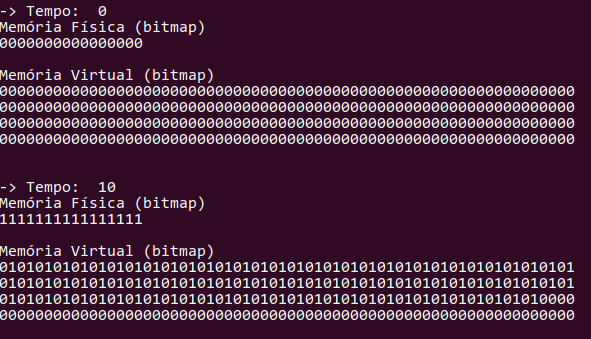
\includegraphics[scale=0.4]{b.png}
		\end{figure}		
	\end{itemize}
\end{frame}

\begin{frame}
	\frametitle{Saída}
	\begin{itemize}
		\item No arquivo de trace foi definido que a memória física teria tamanho 64, a virtual, 1024, e que o tamanho das páginas (s e p) seria 4.
		\item Podemos ver então, no bitmap da memória física, 16 bits (64/4) e no da virtual, 256 (1024/4).
		\item 0 é para posição livre e 1 é para posição ocupada.
		\item Depois disso é mostrado o número de Page Faults do início da execução até o momento exibido.
	\end{itemize}
\end{frame}

\begin{frame}
	\frametitle{Testes}
	\begin{itemize}
		\item Fizemos dois tipos de teste: Número de Page Faults (para comparar os algoritmos de substituição de página) e Tempo de execução (para comparar os algoritmos de gerenciamento de espaço livre).
		\item Para testar, fizemos um script em Python que substitui o módulo ep3.py, e apenas chamava as funções de gerenciador.py com os argumentos necessários, pela quantidade de vezes que fossem precisas.
		\item O número de Page Faults não varia em repetidas execuções, pois os algoritmos são determinísticos.
		\item O tempo de execução varia, pois mesmo que os algoritmos sejam previsíveis, o computador de uso geral mostra variações quando rodamos os comandos.
		\item O arquivo de trace tinha 100 processos que eram simulados em uma memória física de tamanho 64, tamanho virtual 2048, s e p iguais a 4. Cada processo durava no máximo tempo 15.
	\end{itemize}
\end{frame}

\begin{frame}
	\frametitle{Testes}
	\framesubtitle{Page Faults}
	\begin{itemize}
		\item Estes testes foram executados uma vez.
		\item Para testar os diferentes algoritmos de forma justa, fixamos um algoritmo de gerenciamento de espaço livre. No caso, todos foram executados com o First Fit.
		\item Os resultados foram: (legenda para o gráfico a seguir)
		\begin{enumerate}
			\item Optimal: 374 page faults.
			\item Second-Chance: 372 page faults.
			\item Clock: 374 page faults.
			\item LRU: 381 page faults.
		\end{enumerate}
	\end{itemize}
\end{frame}

\begin{frame}
	\begin{figure}[!h]
		\centering
		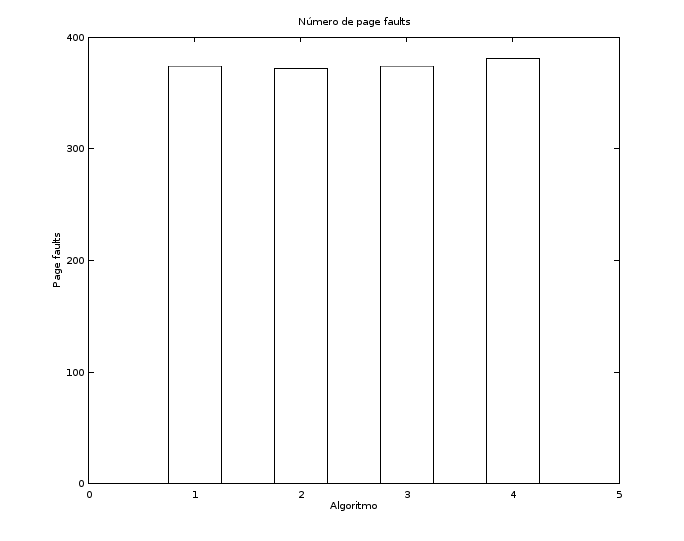
\includegraphics[scale=0.4]{c.png}
	\end{figure}
\end{frame}

\begin{frame}
	\frametitle{Testes}
	\framesubtitle{Tempo de execução}
	\begin{itemize}
		\item Estes testes foram executados trinta vezes.
		\item Para testar os diferentes algoritmos de forma justa, fixamos um algoritmo de substituição de página. No caso, todos foram executados com o Optimal.
		\item Os resultados foram: (legenda para o gráfico a seguir)
		\begin{enumerate}
			\item First Fit: 0.1531049 s - [0.1511358, 0.1550740].
			\item Next Fit: 0.1000248 s - [0.09488377, 0.10516583].
			\item Best Fit: 0.2010095 s - [0.198864, 0.203155].
			\item Worst Fit: 0.2473311 s - [0.2310442, 0.2636181].
		\end{enumerate}
		\item ALGORITMO: MÉDIA DE TEMPO - INTERVALO DE EXECUÇÃO
		\item Não compensava medir cada acesso à memória, por isso calculamos o tempo de execução inteiro.
	\end{itemize}
\end{frame}

\begin{frame}
	\begin{figure}[!h]
		\centering
		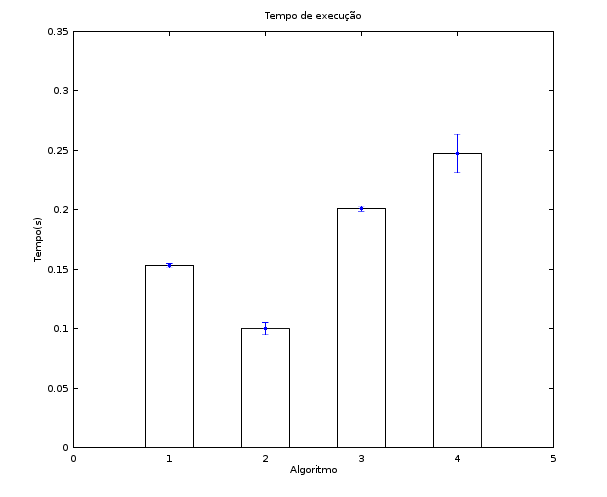
\includegraphics[scale=0.4]{d.png}
	\end{figure}
\end{frame}

\end{document} 